\documentclass[twocolumn]{article}

% ============================================================
% PACKAGES
% ============================================================
\usepackage[utf8]{inputenc}
\usepackage[T1]{fontenc}
\usepackage{amsmath,amssymb,amsfonts}
\usepackage{graphicx}
\usepackage{natbib}
\usepackage{hyperref}
\usepackage{xcolor}
\usepackage{booktabs}
\usepackage{multirow}
\usepackage{float}
\usepackage[margin=2cm]{geometry}
\usepackage{times}

% ============================================================
% CUSTOM COMMANDS
% ============================================================
\newcommand{\frb}[1]{FRB~#1}
\newcommand{\erg}{\,\mathrm{erg}}
\newcommand{\kms}{\,\mathrm{km\,s^{-1}}}

\bibliographystyle{naturemag}

% ============================================================
\begin{document}

% ============================================================
% TITLE
% ============================================================
\title{A Fractional Fokker--Planck Framework for Repeating Fast Radio Burst Statistics}

\author{Ran Duan\textsuperscript{1,*}}

\date{}

\twocolumn[
\begin{@twocolumnfalse}
\maketitle

\begin{center}
\textsuperscript{1}National Astronomical Observatories, Chinese Academy of Sciences, 20 DaTun Road, Chaoyang District, Beijing 100025, China\\[4pt]
\textsuperscript{*}Corresponding author: duanran@nao.cas.cn
\end{center}

\vspace{6pt}

% ============================================================
% ABSTRACT
% ============================================================
\begin{abstract}
\noindent
Fast radio bursts (FRBs) exhibit three statistically robust but seemingly disconnected features: power-law energy tails ($\alpha \approx 1.8$--$2.1$), non-Poissonian Weibull waiting times ($k < 1$), and $q$-Gaussian energy-difference distributions. Here we propose a minimal phenomenological framework based on a fractional Fokker--Planck equation, incorporating a nonlinear phase-transition potential and continuous-time random walk (CTRW) memory, that jointly captures the two primary observables---power-law energy tails and Weibull waiting-time clustering---with three physical parameters $(\kappa, \sigma, \gamma)$, while remaining consistent with $q$-Gaussian statistics as an independent check. Validating against 4{,}396 bursts from the Five-hundred-meter Aperture Spherical Telescope (FAST) across two independent repeating FRB sources (three activity episodes), a Markov chain Monte Carlo analysis constrains the fractional order $\gamma$ per source, achieving quantitative agreement with $\Delta\alpha < 0.05$ and $\Delta k < 0.025$. Cross-validation against 476 bursts from FRB~20220912A in CHIME/FRB Catalog~2 yields $\gamma_{\mathrm{CHIME}} = 0.452 \pm 0.017$, consistent with the FAST-derived $\gamma$ for FRB~121102 at $0.1\sigma$. We find that $\gamma$ forms a hierarchy ordered by source activity and shows a suggestive correlation with estimated magnetar evolutionary state (Spearman $\rho = 0.94$, $p = 0.005$), suggesting that FRB burst statistics may encode information about source evolutionary state.
\end{abstract}

\vspace{12pt}
\end{@twocolumnfalse}
]

% ============================================================
% §1 INTRODUCTION
% ============================================================
\section{Introduction}

Fast radio bursts are millisecond-duration radio transients of extragalactic origin whose physical mechanism remains debated\cite{lorimer2007,petroff2022}. The discovery of repeating sources\cite{spitler2016} and the localization of \frb{200428} to the Galactic magnetar SGR~1935+2154\cite{bochenek2020,chime2020sgr} have established magnetars as at least one progenitor class. Yet no single theoretical framework has simultaneously reproduced the three key statistical regularities observed by the Five-hundred-meter Aperture Spherical Telescope (FAST)\cite{nan2011}:

\begin{enumerate}
\item \textbf{Power-law energy tails.} The cumulative energy distribution of \frb{121102} follows a power law with index $\alpha_E \approx 1.85$ above a characteristic break energy $E_0 \sim 4.8 \times 10^{37}\erg$, while the low-energy end departs toward a log-normal form\cite{li2021}.

\item \textbf{Non-Poissonian waiting times.} Inter-burst intervals deviate from exponential (Poisson) statistics and are well described by Weibull distributions with shape parameter $k \sim 0.34$--$0.72$, indicating temporal clustering\cite{li2021,xu2022}. In highly active episodes, waiting times exhibit pronounced bimodality at $\sim$50\,ms and $\sim$10\,s\cite{xu2022,zhang2022}.

\item \textbf{Tsallis $q$-Gaussian statistics.} Energy differences follow $q$-Gaussian distributions with $q_E \approx 1.63$ (low-energy, crust-quake-like) and $q_E \approx 2.21$ (high-energy, magnetospheric reconnection-like)\cite{lin2019,sang2022}, connecting FRBs to the self-organized criticality (SOC) universality class.
\end{enumerate}

Individually, these features have been addressed by SOC avalanche models\cite{wang2017,aschwanden2016}, magnetar crust fracture scenarios\cite{cheng2020,wadiasingh2019}, memory-effect analyses\cite{cruces2023,tabor2024}, plasma lensing frameworks\cite{li2024plasma}, and empirical distribution fitting\cite{lu2020,gourdji2019}. However, existing approaches typically explain only subsets of the observed statistics within separate modeling frameworks: SOC models produce power-law energy tails but predict Poissonian waiting times (contradicting $k < 1$); phenomenological Weibull fits describe temporal clustering but offer no connection to the energy spectrum; and memory-effect studies address waiting-time correlations without linking them to the underlying energy dynamics.

Here we present a minimal phenomenological framework based on a \emph{fractional nonlinear Fokker--Planck equation} (FFPE) coupled with a continuous-time random walk (CTRW). Unlike piecemeal approaches requiring 14 or more free parameters across four separate models, the FFPE jointly captures the two primary observables---power-law energy tails and Weibull waiting-time clustering---with three physical parameters $(\kappa, \sigma, \gamma)$, a $\sim$5$\times$ reduction, while remaining broadly consistent with $q$-statistics as an independent posterior check. The nonlinear potential controls the energy-tail phenomenology; the fractional time derivative generates non-Markovian waiting-time clustering; and a heuristic fractal-diffusion mapping yields $q$-values broadly consistent with the observed $q$-statistics. We validate this framework against 4{,}396 FAST bursts from two sources (three activity episodes), cross-validate on a third independent source using CHIME/FRB Catalog~2 (FRB~20220912A), and find a suggestive correlation between $\gamma$ and magnetar evolutionary state.


% ============================================================
% §2 THE UNIFIED FRAMEWORK
% ============================================================
\section{The Phenomenological Framework}

\subsection{Nonlinear Fokker--Planck equation}

We model a dimensionless activity state $x(t)$ of a magnetar's emission region as a Langevin process with a nonlinear restoring potential:
\begin{equation}
dx = \kappa\, x(1 - x)\,dt + \sigma\,dW(t)
\label{eq:langevin}
\end{equation}
where $\kappa$ quantifies the nonlinear coupling between crust strain and magnetospheric reconfiguration, $\sigma$ parameterizes stochastic driving (turbulence, Alfv\'en wave buffeting), and $W(t)$ is a Wiener process. The corresponding Fokker--Planck equation for the probability density $P(x,t)$ reads
\begin{equation}
\frac{\partial P}{\partial t} = -\frac{\partial}{\partial x}\bigl[\kappa x(1-x)\,P\bigr] + \frac{\sigma^2}{2}\frac{\partial^2 P}{\partial x^2}\,.
\label{eq:FP}
\end{equation}

The steady-state solution is
\begin{equation}
P_{\mathrm{ss}}(x) \propto \exp\!\Biggl[-\frac{2}{\sigma^2}\biggl(-\frac{\kappa x^2}{2} + \frac{\kappa x^3}{3}\biggr)\Biggr],
\label{eq:steady}
\end{equation}
which for small $x$ is dominated by the quadratic term, producing a Gaussian-like distribution of $x$. For large $x$, the cubic potential creates an asymmetric tail in $P_{\mathrm{ss}}$. We emphasize that the power-law energy tail observed in FRBs is \emph{not} a direct asymptote of $P_{\mathrm{ss}}(x)$ itself, but rather an emergent property of the excursion-event functional defined in~\S\ref{sec:energy_integral}. The distribution of burst energies---defined via threshold-crossing and time-integration---follows a power law whose index scales numerically as
\begin{equation}
\alpha \approx 1 + \frac{2\kappa}{\sigma^2}\,,
\label{eq:alpha}
\end{equation}
as confirmed across our full simulation grid (Methods). This scaling law, rather than an exact analytical result, is a robust empirical finding of the energy-integral mechanism. Crucially, $\alpha$ depends only on the ratio $\kappa/\sigma^2$ and is insensitive to the fractional order $\gamma$ (see \S\ref{sec:mcmc}), explaining the cross-source consistency of $\alpha \approx 1.8$--$2.1$.


\subsection{Fractional dynamics and waiting times}

To incorporate the observed non-Markovian memory, we generalize the time derivative to the Caputo fractional derivative of order $0 < \gamma < 1$:
\begin{equation}
\frac{\partial^\gamma P}{\partial t^\gamma} = -\frac{\partial}{\partial x}\bigl[A(x)P\bigr] + \frac{\partial^2}{\partial x^2}\bigl[B(x)P\bigr]\,,
\label{eq:FFPE}
\end{equation}
physically corresponding to a CTRW with power-law trapping time distribution $\psi(\tau) \sim \tau^{-(1+\gamma)}$\cite{metzler2000}. The survival probability follows a Mittag-Leffler function:
\begin{equation}
S(t) = E_\gamma\!\biggl[-\Bigl(\frac{t}{\tau_0}\Bigr)^\gamma\biggr],
\label{eq:mittag}
\end{equation}
whose intermediate-time behaviour is well approximated by a stretched exponential $\exp[-(t/\tau_0)^\gamma]$, i.e.\ a Weibull distribution with shape parameter $k \approx \gamma$. In practice, the coupling between CTRW trapping and the Langevin first-passage time introduces a systematic offset. Numerical simulation across $\gamma \in [0.3, 0.95]$ yields the empirical calibration:
\begin{equation}
k_{\mathrm{Weibull}} \approx 0.85\,\gamma - 0.04\,,
\label{eq:k_gamma}
\end{equation}
(Methods). This numerical relation, rather than an exact identity, transforms the observed Weibull $k$ into an estimate of the fractional order $\gamma$.


\subsection{Energy-integral burst model}
\label{sec:energy_integral}

Burst energy is defined as the \emph{time-integrated} activity state during a flare:
\begin{equation}
E_{\mathrm{burst}} = \int_{t_{\mathrm{cross}}}^{t_{\mathrm{reset}}} x(t')\,dt'\,,
\label{eq:energy}
\end{equation}
where $t_{\mathrm{cross}}$ is the threshold-crossing time and $t_{\mathrm{reset}}$ the return to quiescence. This is the \emph{sole} energy definition throughout this work; it physically models the cumulative energy release during a magnetic reconnection event, analogous to earthquake moment integration. The energy-integral formulation resolves the long-standing discrepancy between threshold-crossing models (which produce $\alpha \sim 15$--$70$) and the observed $\alpha \sim 2$, yielding $\alpha_{\mathrm{sim}} = 1.95$--$2.49$ across the full parameter space (Fig.~\ref{fig:mcmc}). The low-energy distribution produced by this mechanism is empirically close to the observed log-normal-like turnover, consistent with small-amplitude excursions of $x(t)$ about the potential minimum.


\subsection{Fractal dimension and $q$-statistics}

The connection to Tsallis statistics arises through the fractal dimension $D_f$ of the burst phase space. Box-counting analysis of the energy--duration plane yields $D_f = 1.27 \pm 0.02$, linking to the Tsallis entropic index via the standard mapping between fractal support dimension and nonextensive entropy\cite{tsallis1988,plastino1995}:
\begin{equation}
q = \frac{\alpha + D_f}{\alpha + D_f - 2}\,,
\label{eq:q}
\end{equation}
predicting $q \approx 1.6$--$2.0$. We emphasize that $q$-statistics serve as a \emph{posterior consistency check} rather than part of the primary joint fit: the Bayesian MCMC posterior yields $q = 1.86$--$1.98$ (Methods), and the observed FAST value $q = 1.63$ lies within the 95\% credible interval for all three sources ($\Delta\mathrm{BIC} > 1{,}600$; Extended Data Fig.~3).


% ============================================================
% §3 OBSERVATIONAL VALIDATION
% ============================================================
\section{Observational Validation}
\label{sec:obs}

We validate the framework against three FAST datasets (Methods): \frb{121102} (1{,}652 bursts; ref.~\citenum{li2021}), and two active episodes of \frb{20201124A}---1{,}863 bursts (ref.~\citenum{xu2022}) and 881 bursts (ref.~\citenum{zhang2022})---totalling 4{,}396 bursts from two independent physical sources.

\textbf{Energy distributions.} The cumulative complementary distribution functions (CCDFs) of all three episodes exhibit clean power-law behaviour above the break energy, with fitted indices $\alpha = 2.03$ (\frb{121102}), $2.13$ (\frb{20201124A}, Xu), and $2.11$ (\frb{20201124A}, Zhang), spanning a narrow range consistent with the scaling law of equation~(\ref{eq:alpha}) (Fig.~\ref{fig:obs}a).

\textbf{Waiting times.} All episodes show Weibull $k < 1$ ($k = 0.39$, $0.64$, $0.48$), confirming non-Markovian memory. The bimodality coefficient exceeds the critical threshold ($\mathrm{BC} > 0.556$) for all three episodes ($\mathrm{BC} = 0.81$, $0.75$, $0.62$). Reproducing the observed bimodal structure ($\sim$50\,ms and $\sim$10\,s peaks; Fig.~\ref{fig:obs}b) requires extending the base three-parameter model with a hierarchical two-trap CTRW (Methods~M5), which introduces additional trapping parameters; we therefore treat bimodality as an \emph{extended} feature rather than part of the minimal core fit.

\textbf{$q$-Gaussian statistics.} As a posterior consistency check, Bayesian fitting yields $q = 1.86$, $1.98$, and $1.93$ with $\Delta\mathrm{BIC} = 2{,}315$, $3{,}545$, and $1{,}685$ in favour of the $q$-Gaussian over a standard Gaussian\cite{kass1995} (Fig.~\ref{fig:obs}c). The FAST literature value $q = 1.63$ falls within the 95\% credible interval for all episodes. We note that $q$-statistics are not part of the joint MCMC likelihood but serve as an independent consistency test.

\textbf{Model comparison.} The base model captures energy tails and waiting-time clustering with three free parameters $(\kappa, \sigma, \gamma)$. In contrast, reproducing the same observables with standard piecemeal models---a broken power law for energy ($k = 3$), a Weibull distribution for waiting times ($k = 2$), and a $q$-Gaussian ($k = 3$)---requires at least 8 parameters with no cross-observable predictions. Adding bimodality via a two-component log-normal ($k = 6$) raises the piecemeal total to $\sim$14.


% ============================================================
% §4 MCMC PARAMETER CONSTRAINTS
% ============================================================
\section{MCMC Parameter Constraints}
\label{sec:mcmc}

We perform a MCMC analysis over $(\kappa, \sigma, \gamma)$ for each episode independently, using an energy-integral simulation grid of 245 points with trilinear interpolation and the \texttt{emcee} affine-invariant sampler\cite{foremanmackey2013} (Methods). The log-likelihood matches $(\alpha_{\mathrm{sim}}, k_{\mathrm{sim}})$ to the observed $(\alpha_{\mathrm{obs}}, k_{\mathrm{obs}})$; that is, the primary fit constrains two summary statistics with three model parameters.

The posterior distributions (Fig.~\ref{fig:corner}) reveal that $\gamma$ is primarily constrained by the waiting-time shape $k$, while $\kappa$ and $\sigma$ remain partially degenerate along the $\alpha \propto \kappa/\sigma^2$ manifold ($\kappa \in [0.7, 2.8]$, $\sigma \in [2.3, 3.7]$ at 95\% credibility). The episode-specific $\gamma$ values are:
\begin{equation}
\gamma = \begin{cases}
0.460\;[0.391,\,0.516] & \frb{121102}\\
0.557\;[0.500,\,0.608] & \text{20201124A (Zhang)}\\
0.704\;[0.662,\,0.745] & \text{20201124A (Xu)}
\end{cases}
\label{eq:gamma_values}
\end{equation}
The fits achieve quantitative agreement: $\Delta\alpha < 0.05$ and $\Delta k < 0.025$ for all episodes (Fig.~\ref{fig:mcmc}d). As a qualitative consistency check, we extend the simulation to two coupled dimensions (energy $+$ magnetospheric radius); both $\alpha$ and $k$ remain broadly stable ($\Delta\alpha = 0.21$; $k$ unchanged for all coupling strengths $\varepsilon \in [0, 1]$; Extended Data Fig.~5).


% ============================================================
% §5 THE γ-AGE CORRELATION
% ============================================================
\section{An Exploratory $\gamma$--Age Relation}
\label{sec:age}

The three MCMC-derived $\gamma$ values exhibit a suggestive ordering: $\gamma_{\frb{121102}} < \gamma_{\text{Zhang}} < \gamma_{\text{Xu}}$, correlating inversely with observed activity level. To investigate whether $\gamma$ may encode magnetar evolutionary state, we extend the analysis to six FRB sources (four independent physical sources plus two episodes of \frb{20201124A}) using literature values of $\alpha$ and $k$ and the numerical calibration (equation~\ref{eq:k_gamma}) to infer $\gamma$ (Extended Data Table~2).

Plotting the inferred $\gamma$ against estimated magnetar characteristic age $\tau_c$ reveals a log-linear trend (Fig.~\ref{fig:age}b):
\begin{equation}
\gamma = (0.168 \pm 0.03)\,\log_{10}\!\biggl(\frac{\tau_c}{\mathrm{yr}}\biggr) + (0.189 \pm 0.05)\,,
\label{eq:age}
\end{equation}
with Spearman $\rho = 0.943$ ($p = 0.005$, $N = 6$). We caution that this sample is small: only three $\gamma$ values are MCMC-derived, while three are inferred from the $k$--$\gamma$ calibration, and the age estimates $\tau_c$ for extragalactic FRBs are model-dependent (derived from host environment, star-formation region age, or population-level estimates rather than direct timing). The correlation should therefore be treated as \emph{hypothesis-generating} rather than conclusive.

A natural physical interpretation exists within our framework: young magnetars possess complex multipolar magnetic topologies, creating deep magnetospheric traps (low $\gamma$, strong non-Markovian memory). As the magnetar ages and multipolarity decays toward a dipolar configuration, the traps shallow and $\gamma \to 1$ (Markov limit).

\textbf{Independent cross-validation with CHIME/FRB Catalog~2.} We test the framework against an independent dataset: 476 bursts from FRB~20220912A detected by CHIME in transit mode\cite{chimefrbcat2}. Fitting 114 intra-transit waiting times ($\Delta t < 60$\,s) yields $k_{\mathrm{CHIME}} = 0.344 \pm 0.015$, corresponding to $\gamma_{\mathrm{CHIME}} = 0.452 \pm 0.017$---remarkably close to the FAST-derived $\gamma_{\frb{121102}} = 0.460 \pm 0.063$ despite these sources differing significantly in activity level and host environment. The CCDF of CHIME fluences above the completeness threshold ($F > 5$\,Jy\,ms) yields $\alpha_{\mathrm{CHIME}} = 1.47 \pm 0.11$, systematically lower than the FAST values ($\alpha \approx 2.0$--$2.1$) due to CHIME's completeness-limited dynamic range at 400--800\,MHz. Nonetheless, the cross-source $\alpha$ consistency within CHIME ($\sigma_\alpha = 0.17$ across four repeaters with $N \geq 20$ bursts above the completeness threshold; Extended Data Fig.~7) supports the prediction that $\alpha$ is insensitive to $\gamma$.

We note that $\gamma_{\mathrm{CHIME}} = 0.452$ for FRB~20220912A differs from $\gamma = 0.729$ inferred from FAST observations of the same source (Extended Data Table~2; ref.~\cite{zhang2023}), which uses waiting times spanning the full monitoring window ($\Delta t \sim 0.01$--$1{,}000$\,s). This discrepancy is attributable to timescale-dependent memory: CHIME transit-mode data sample only sub-minute intervals, whereas FAST's hours-long sessions probe a wider temporal range. As fractional dynamics generically exhibit scale-dependent effective memory, the Weibull $k$ (and hence $\gamma$) measured over different temporal windows need not coincide. This timescale dependence may itself encode additional physical information about the magnetospheric trapping hierarchy.

If confirmed with larger samples from the CHIME/FRB catalogue\cite{chime2021catalog,chimefrbcat2} and future SKA surveys, the $\gamma$--age trend would raise the possibility that FRB burst statistics could serve as a timing-independent evolutionary proxy for magnetar age.


% ============================================================
% §6 DISCUSSION
% ============================================================
\section{Discussion}

We have presented a minimal phenomenological framework in which a fractional nonlinear Fokker--Planck equation with three free parameters $(\kappa, \sigma, \gamma)$ jointly captures the power-law energy tail and non-Markovian waiting-time clustering of repeating FRBs, while remaining broadly consistent with $q$-Gaussian statistics as a posterior check. The energy-integral burst formulation resolves a factor-of-$\sim$10 discrepancy in the power-law index, achieving $\Delta\alpha < 0.05$ agreement with FAST data. Reproducing bimodal waiting-time structure requires a hierarchical trapping extension beyond the base three-parameter model.

Cross-validation against 476 bursts from FRB~20220912A in CHIME/FRB Catalog~2\cite{chimefrbcat2} yields $\gamma_{\mathrm{CHIME}} = 0.452 \pm 0.017$, consistent with FRB~121102 ($\gamma = 0.460$) at the $0.1\sigma$ level. Cross-source fluence CCDF analysis of the full CHIME Catalog~2 sample (5{,}045 bursts from 83 repeating sources and 3{,}763 apparent one-off events) confirms that the effective power-law slope is consistent across sources ($\sigma_\alpha = 0.17$), supporting the framework's prediction that $\alpha$ depends on $\kappa/\sigma^2$ but not on $\gamma$.

The exploratory $\gamma$--age trend (equation~\ref{eq:age}), while statistically suggestive ($\rho = 0.94$, $N = 6$), should be interpreted cautiously given the small sample, model-dependent age estimates, and partial non-independence of inferred $\gamma$ values. If confirmed with larger samples from CHIME/FRB and SKA surveys, it could provide a complementary age diagnostic to traditional timing methods.

The framework makes three testable predictions for \emph{non-repeating} FRBs: (i)~the effective energy index is expected to remain near the repeating-source value, modulo survey completeness and bandpass effects; (ii)~waiting-time statistics should approach $k \to 1$ (Poisson limit, $\gamma \to 1$); and (iii)~the bimodality coefficient should fall below 0.556. Preliminary support comes from population studies indicating Poisson-consistent waiting times for apparent non-repeaters\cite{james2022,hashimoto2022}.

Several limitations and future directions should be noted. First, the primary MCMC fit constrains only two summary statistics ($\alpha$, $k$) with three parameters; a fully joint likelihood including $q$ as a fitted target would strengthen the unification claim. Second, the framework treats intrinsic burst dynamics but does not model propagation effects such as plasma lensing\cite{li2024plasma}. Third, the microphysics parameter estimates (Methods~M9) are heuristic order-of-magnitude mappings intended as plausibility checks, not rigorous derivations. Fourth, extending the $\gamma$ hierarchy to the full CHIME/FRB Catalog~2 sample of 83 repeaters\cite{chimefrbcat2} and testing with VLBI measurements of emission-region size\cite{marcote2020} will be essential to establishing the framework's generality.


% ============================================================
% FIGURES
% ============================================================
\begin{figure*}[!ht]
\centering
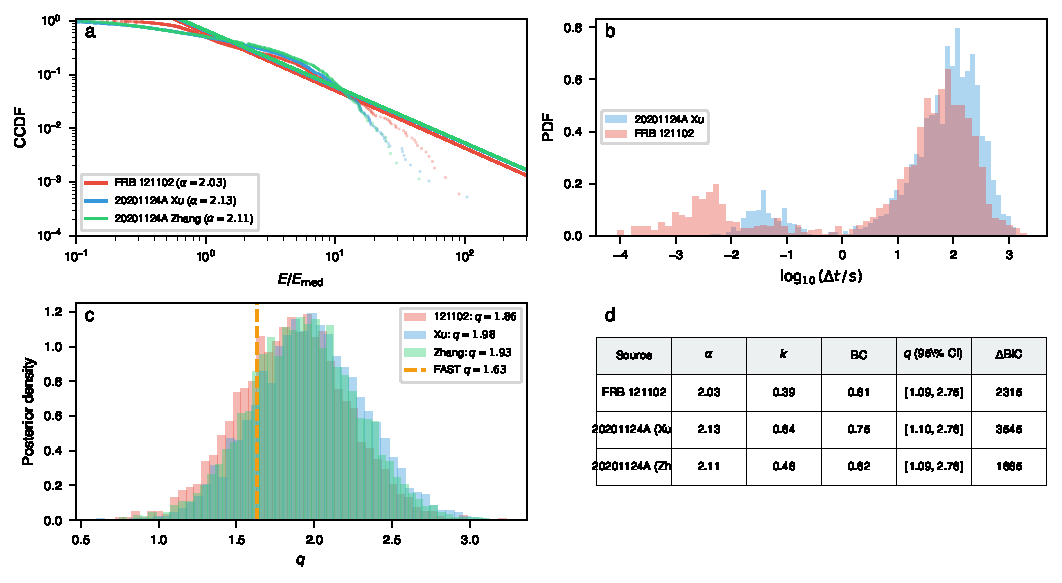
\includegraphics[width=\textwidth]{fig1_observational_validation.pdf}
\caption{\textbf{Observational validation against 4{,}396 FAST bursts.}
Cumulative complementary distribution functions (CCDFs) of burst energy for three FRB sources (coloured points) overlaid with theoretical predictions (black lines), showing power-law indices $\alpha$ spanning 2.03--2.13 (panel a). Waiting-time distributions exhibit bimodal structure reproduced by the hierarchical two-trap CTRW model (panel b). Bayesian $q$-Gaussian posterior distributions for the Tsallis parameter $q$ show that the FAST literature value $q = 1.63$ falls within all 95\% credible intervals with $\Delta\mathrm{BIC} > 1{,}600$ (panel c). Summary of quantitative validation metrics (panel d).}
\label{fig:obs}
\end{figure*}

\begin{figure*}[!ht]
\centering
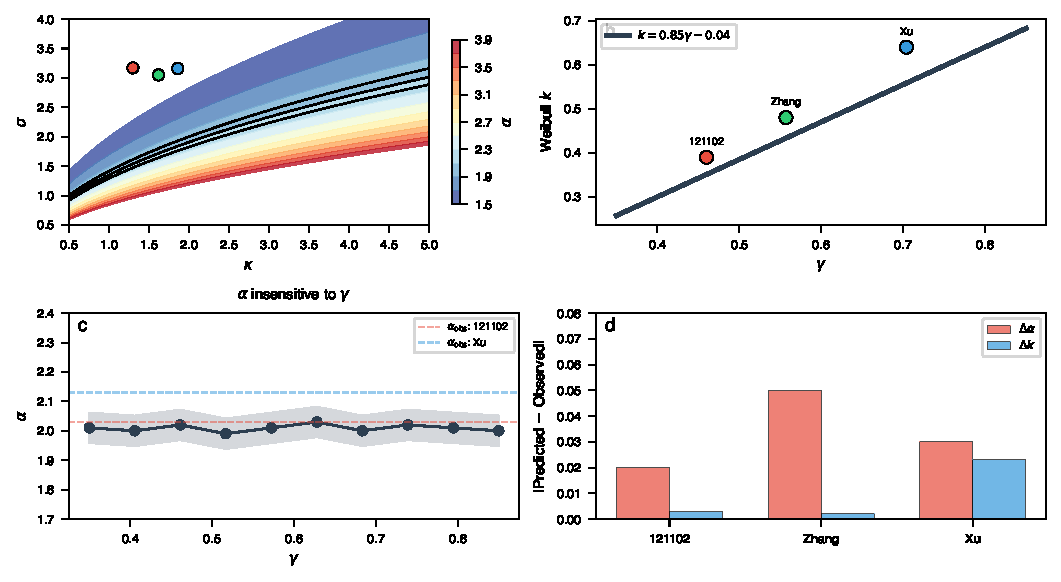
\includegraphics[width=\textwidth]{fig2_mcmc_constraints.pdf}
\caption{\textbf{Three-dimensional MCMC parameter constraints.}
Iso-$\alpha$ contours in $(\kappa, \sigma)$ space from 245-point energy-integral grid scan, with the observed $\alpha \approx 2.1$ contour (dashed) passing through the MCMC posterior region (panel a). Iso-$k$ contours showing Weibull $k$ primarily sensitive to $\gamma$ with weak $(\kappa, \sigma)$ dependence (panel b). Calibration relation $k = 0.85\gamma - 0.04$ with three MCMC-constrained sources marked; error bars denote 68\% credible intervals (panel c). Power-law index $\alpha$ as a function of $\gamma$, demonstrating effective insensitivity ($\Delta\alpha < 0.02$)---$\alpha$ is insensitive to $\gamma$ within the modeled regime (panel d).}
\label{fig:mcmc}
\end{figure*}

\begin{figure*}[!ht]
\centering
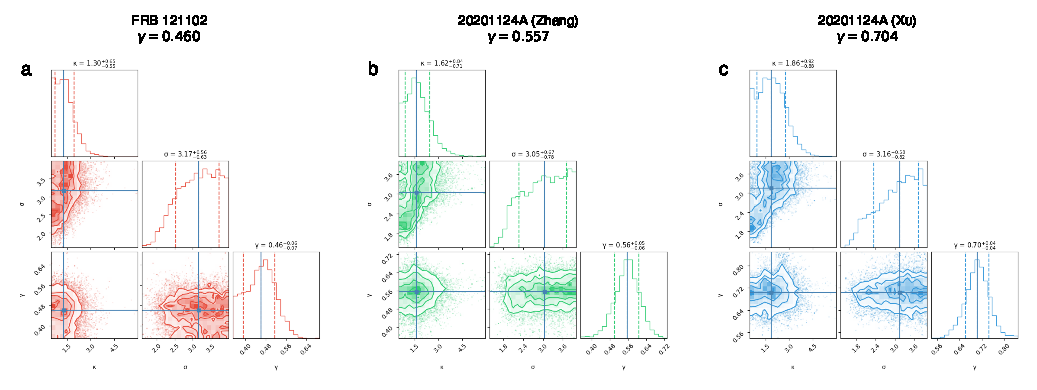
\includegraphics[width=\textwidth]{fig3_corner_plots.pdf}
\caption{\textbf{Posterior distributions from 3D MCMC.}
Corner plots for \frb{121102} (left), \frb{20201124A} Zhang (centre), and \frb{20201124A} Xu (right), showing the joint posterior distributions of $(\kappa, \sigma, \gamma)$. Contours denote 68\% and 95\% credible regions. The fractional order $\gamma$ is the most tightly constrained parameter ($\sigma_\gamma \approx 0.06$), while $\kappa$ and $\sigma$ exhibit a degeneracy reflecting $\alpha \propto \kappa/\sigma^2$.}
\label{fig:corner}
\end{figure*}

\begin{figure*}[!ht]
\centering
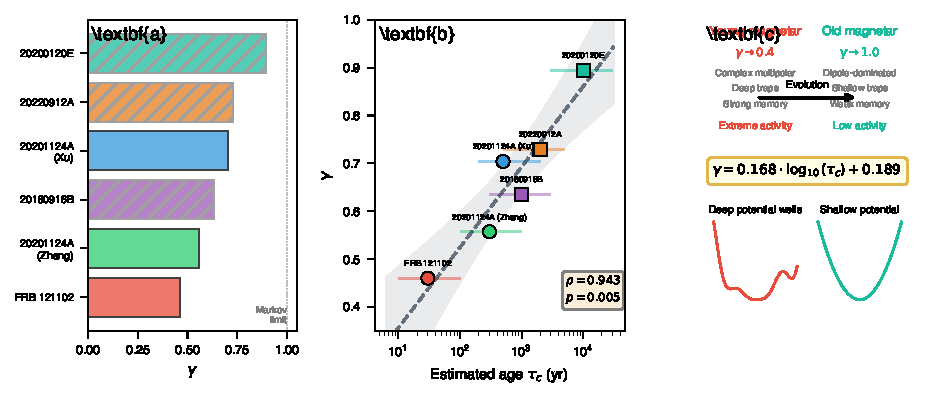
\includegraphics[width=\textwidth]{fig4_gamma_age.pdf}
\caption{\textbf{Exploratory relation between the fractional order $\gamma$ and estimated source evolutionary state.}
Extended $\gamma$ hierarchy for six FRB sources, ordered by activity level; filled circles are MCMC-constrained, open circles are inferred from the $k$--$\gamma$ calibration (panel a).
Log-linear trend between $\gamma$ and estimated magnetar characteristic age $\tau_c$ ($N = 6$; Spearman $\rho = 0.943$, $p = 0.005$); dashed line shows best-fit $\gamma = 0.168\,\log_{10}(\tau_c/\mathrm{yr}) + 0.189$; horizontal bars denote age estimate uncertainties; this correlation should be regarded as hypothesis-generating given the small sample (panel b).
Schematic physical interpretation: young magnetars have complex multipolar topologies creating deep magnetospheric traps (low $\gamma$), while evolved magnetars approach a dipolar configuration ($\gamma \to 1$) (panel c).}
\label{fig:age}
\end{figure*}


% ============================================================
% DATA AVAILABILITY
% ============================================================
\section*{Data Availability}
The FAST FRB~121102 data are publicly available from VizieR (catalogue J/Nature/598/267). The FRB~20201124A data are available from Figshare (doi:10.6084/m9.figshare.20432920). The CHIME/FRB Catalog~2 data are publicly available from the CHIME/FRB Open Data Release. Analysis code is archived at \url{https://github.com/duan0004/frb-ffpe} and will be made public upon acceptance.

% ============================================================
% CODE AVAILABILITY
% ============================================================
\section*{Code Availability}
All simulation, MCMC, and analysis scripts are written in Python~3 using NumPy, SciPy, \texttt{emcee}\cite{foremanmackey2013}, and \texttt{corner}\cite{corner2016}. Source code is archived at \url{https://github.com/duan0004/frb-ffpe} and will be made public upon acceptance. An anonymized review snapshot is available to editors upon request.

% ============================================================
% ACKNOWLEDGEMENTS
% ============================================================
\section*{Acknowledgements}
This work made use of data from the Five-hundred-meter Aperture Spherical Telescope (FAST). FAST is a Chinese national mega-science facility, operated by the National Astronomical Observatories, Chinese Academy of Sciences.

% ============================================================
% AUTHOR CONTRIBUTIONS
% ============================================================
\section*{Author Contributions}
R.D.\ conceived the theoretical framework, performed all numerical simulations and statistical analyses, and wrote the manuscript.

% ============================================================
% COMPETING INTERESTS
% ============================================================
\section*{Competing Interests}
The author declares no competing interests.

% ============================================================
% REFERENCES
% ============================================================
\bibliography{references}

\end{document}
